\label{sec:futureTopics}
Beyond the topics discussed in this study, further ideas led to several additional, mostly incomplete implementations of tools to further investigate eddy dynamics via automated tracking. The following are a handful of examples of topics to address subsequent to this work.

%%....................................F.I.G.U.R.E.............................................
\begin{figure}
	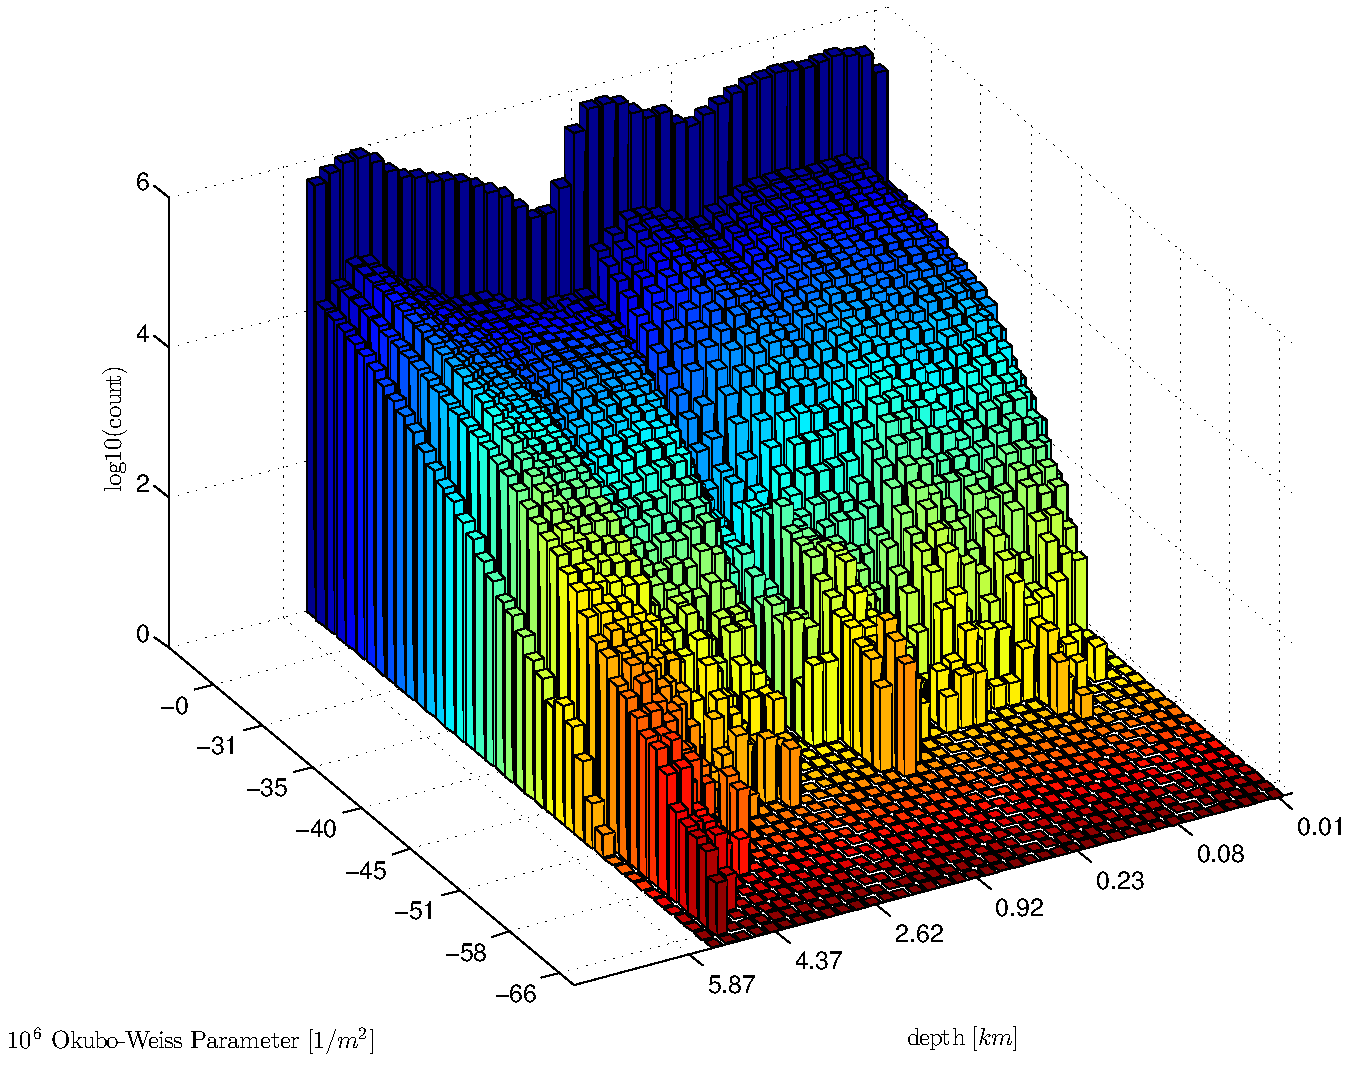
\includegraphics[]{OW_count-OW-depth}
	\caption{Histogram of global $\okubo$ as a function of depth calculated from \POP~current~vectors. The idea was to find the surface $z_{ow}(y,x)$ of maximum $-\okubo(z,y,x)$ and then use that depth as the depth to take the mean current from (see \cref{sec:netU}). The maximum tends to be at the ocean floor which led to the conjecture that the numerical implementation of $\okubo$ might have been erroneous. Further application was hence abandoned.  }
	\label{fig:OW_count-OW-depth}
\end{figure}
%%....................................F.I.G.U.R.E.............................................


\begin{itemize}
\setlength\itemsep{2mm}
\item
\textbf{Applying the algorithm at different depths}\\
One advantage of using model data is that it is not limited to the sea surface. All parameters are also available for all of the vertical levels. In order to apply the same algorithm that was used for \SSH~at depth, barotropic pressure plus density integrals were used to construct virtual \textit{SSH} anomalies for different depths. Preliminary results were promising and seemed to agree well with the findings by \citet{Petersen2013} with respect to the regional distribution of eddy-\textit{thicknesses}. Since the necessary temperature- and salt-data were available for merely 2 years and because computational resources were first and foremost needed for the surface-analyses, this chapter was abandoned entirely for now.
The three-dimensional structure should certainly be the focus from here on, as its physics are thus far neither well observed nor understood. \Citeauthor{Petersen2013} \eg note that even though the majority of long-lived eddies do extend all the way to the surface, still \textit{thousands} of tall, sub-surface eddies exist that remain hidden from any sea-surface based detection method. And quoting \citep{Zhang2013}: \textit{Further study in refining this [vertical] structure is expected, and the refined structure can serve as a benchmark for numerical models where mesoscale eddies are explicitly resolved. In addition, the generation mechanism for this universal structure remains unknown; thus, exploring such mechanism may bring new excitement to eddy research.} \\

\item
\textbf{Influence of mean flow on translational speeds.}\\
Knowledge of the vertical scale is also indispensable for investigations of the effect of mean current on eddy dynamics. A considerable amount of time was wasted (to no avail), trying to find vertical local maxima of $-\okubo$ in order to help construct a mean-flow surface taken from respective depths (see \cref{fig:OW_count-OW-depth}).
The idea here was that the depth of strongest $-\okubo$ would be the depth of strongest eddy activity.\\
Under the assumption that the observed speeds are in fact simply the sum of theoretical long Rosbby-wave phase speeds plus the mean flow \ie simple Doppler-shift, another approach would be to look for respective best-fitting depth-range to average the mean-flow over. \Ie seek $z_{1}(y,x),\; z_{2}(y,x)$ that yield the minimum to
\begin{equation}
c_{rossby,long,x}
+
\frac{1}{\delta z} \int_{z_{1}}^{z_{2}} u_{meanFlow}(z,y,x) \; \mathrm{d}z
-
u_{observed}
\end{equation}
Where $z_{2}$ would likely be the surface.
\item
\textbf{Tracers}\\
As mentioned in \cref{section:lengthoftracks}, it should be interesting to not only track peaks of \SSH~anomaly, but parallelly also \eg drop virtual buoys into the centers of eddies and then calculate their positions incrementally from the available current vectors (model only of course). Or simpler, look at basic T/S-watermass characteristics (and their variability) of eddy cores as a function of time. Both could on the one hand illuminate to what degree and under which circumstances the eddy is to be interpreted as a material, water-mass transporting vortex as opposed to an immaterial, linear Rossby-wave, and on the other hand help to pin-point mistakes of the tracking algorithm.

\item
\textbf{Track Paths}\\
Eddy tracks appear to be influenced by bathymetry. Drawing tracks over a map of \eg $N H/f$ or $H/f$ contours could further clarify the influence of bathymetry and density gradients on the lateral propagation of eddies.

%\item
%\textbf{profiles}\\
%(see \cref{fig:gaussVSquadSmaller})

\item
\textbf{Rhines Scale}\\
It would be interesting to compare the tropical eddy scales to the local Rhines scale ($\Lb$) and test whether the theory of the two regimes mentioned by \citet{Eden2007} can be supported.

\end{itemize}




\begin{figure*}
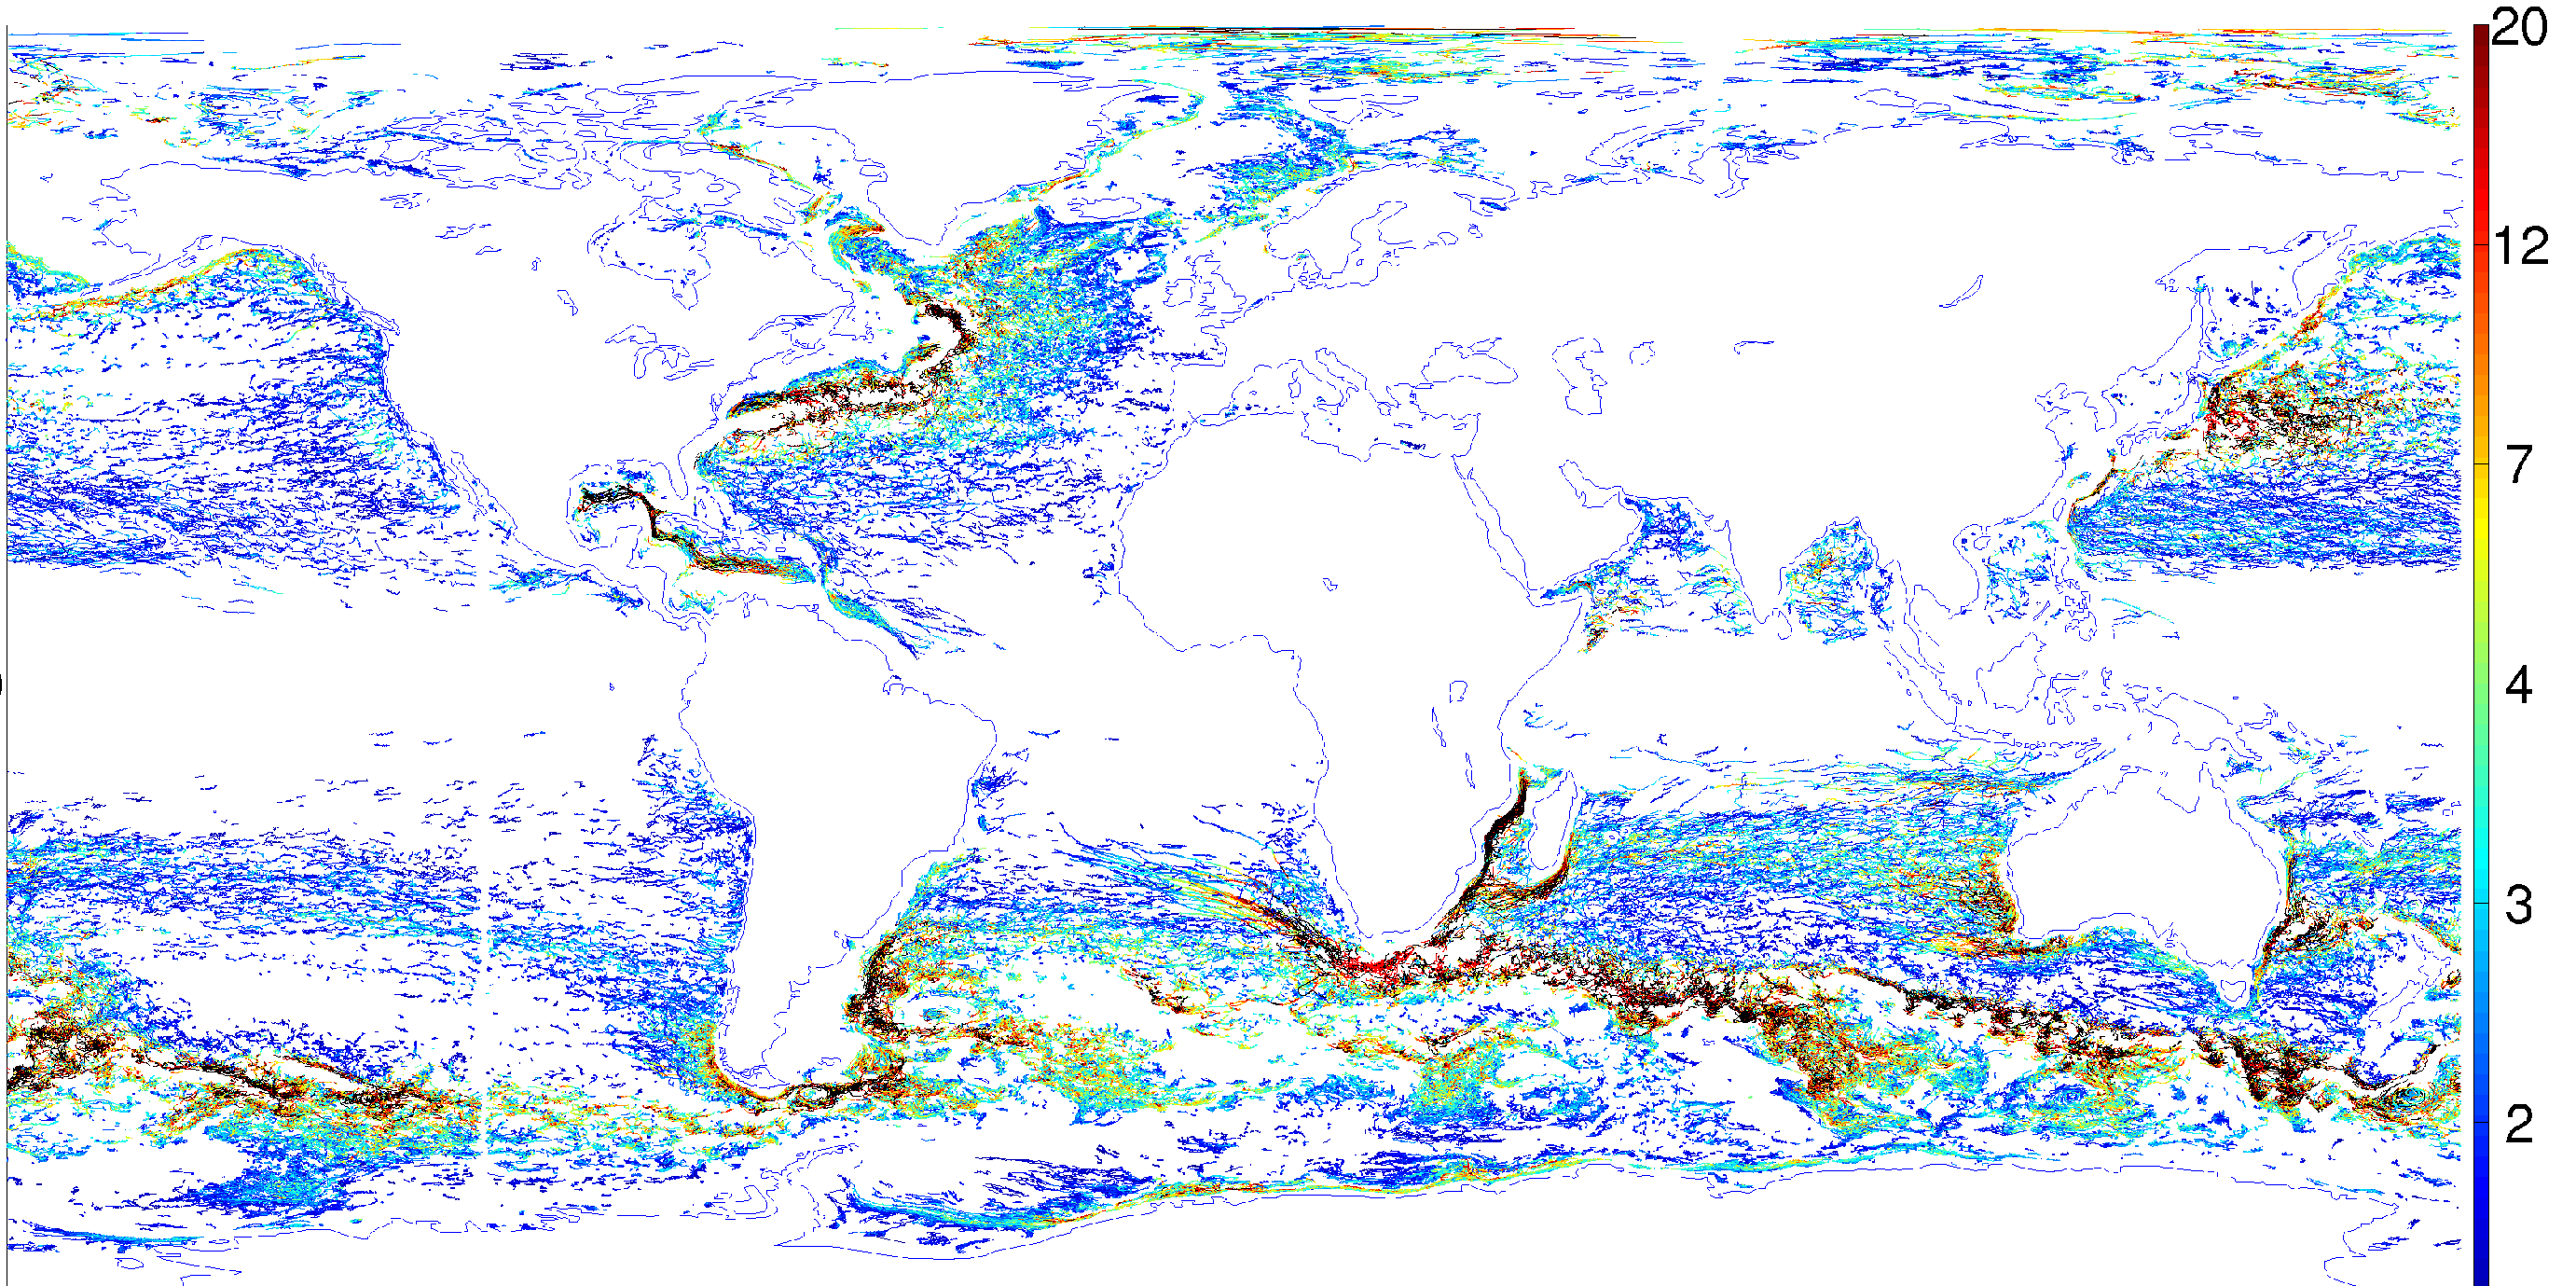
\includegraphics[]{TrackPeakampto_ellipseAntiCycsCrpd}
\caption{Amplitude $\Unit{\si{\cm}}$ (w.r. to contour). Tracks are from very early \POP~test-runs (Note how tracking across zonal edge of the data was not implemented yet).}
\label{fig:TrackPeakampto_ellipseAntiCycsCrpd}
\end{figure*}
